\documentclass[crop, tikz]{standalone}
\usepackage{tikz}
\usepackage{amsmath}
\usepackage{amssymb}
\usepackage{xcolor}

\usetikzlibrary{positioning, decorations.pathmorphing}

\definecolor{olivegreen}{rgb}{0,0.6,0}

\begin{document}
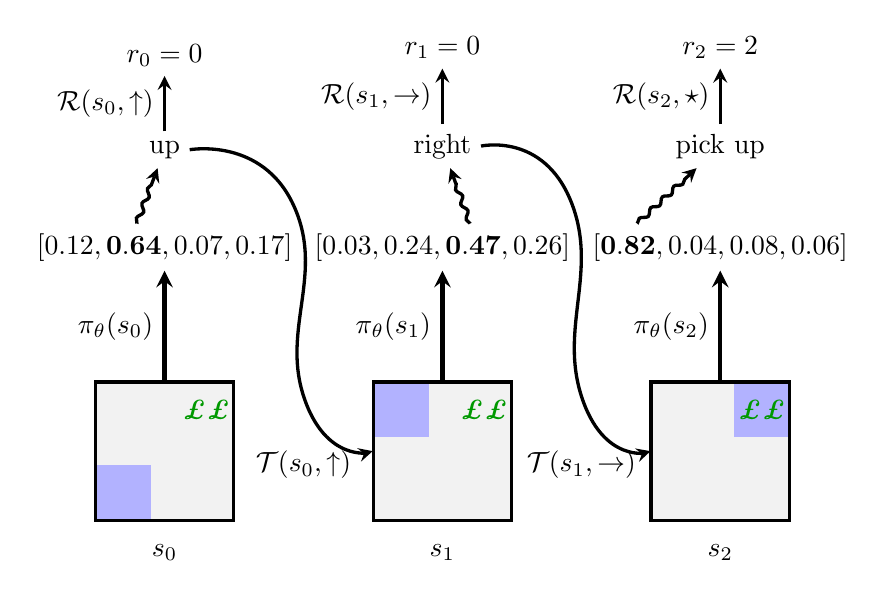
\begin{tikzpicture}
	\node[rectangle, minimum width=5em, minimum height=5em, fill=lightgray!20] (X) {};
	\node[rectangle, fill=blue!30, minimum width=2em, minimum height=2em, xshift=-1.5em, yshift=-1.5em] at (X) (AA) {};
	\node[rectangle, minimum width=2em, minimum height=2em, xshift=1.5em, yshift=1.5em, olivegreen] at (X) (LA) {$\boldsymbol\pounds\boldsymbol\pounds$};
	\node[rectangle, very thick, draw, minimum width=5em, minimum height=5em] at (X) (K) {};
	\node[rectangle, right=5em of X, minimum width=5em, minimum height=5em, fill=lightgray!20] (Y) {};
	\node[rectangle, fill=blue!30, minimum width=2em, minimum height=2em, xshift=-1.5em, yshift=1.5em] at (Y) (BB) {};
	\node[rectangle, minimum width=2em, minimum height=2em, xshift=1.5em, yshift=1.5em, olivegreen] at (Y) (LB) {$\boldsymbol\pounds\boldsymbol\pounds$};
	\node[rectangle, very thick, draw, minimum width=5em, minimum height=5em] at (Y) (W) {};
	\node[rectangle, right=5em of Y, minimum width=5em, minimum height=5em, fill=lightgray!20] (Z) {};
	\node[rectangle, fill=blue!30, minimum width=2em, minimum height=2em, xshift=1.5em, yshift=1.5em] at (Z) (CC) {};
	\node[rectangle, minimum width=2em, minimum height=2em, xshift=1.5em, yshift=1.5em, olivegreen] at (Z) (LC) {$\boldsymbol\pounds\boldsymbol\pounds$};
	\node[rectangle, very thick, draw, minimum width=5em, minimum height=5em] at (Z) (AS) {};
		
	\node[below=0.5em of X] (l1) {$s_0$};
	\node[below=0.5em of Y] (l2) {$s_1$};
	\node[below=0.5em of Z] (l3) {$s_2$};
		
	\node[above=4em of X] (P1) {$[0.12, {\bf 0.64}, 0.07, 0.17]$};
	\node[above=4em of Y] (P2) {$[0.03, 0.24, {\bf 0.47}, 0.26]$};
	\node[above=4em of Z] (P3) {$[{\bf 0.82}, 0.04, 0.08, 0.06]$};
		
	\draw[-stealth, ultra thick] (X) -- node[left] {$\pi_\theta(s_0)$} (P1);
	\draw[-stealth, ultra thick] (Y) -- node[left] {$\pi_\theta(s_1)$} (P2);
	\draw[-stealth, ultra thick] (Z) -- node[left] {$\pi_\theta(s_2)$} (P3);
		
	\node[above=2em of P1] (A1) {up};
	\node[above=2em of P2] (A2) {right};
	\node[above=2em of P3] (A3) {pick up};
		
	\draw[-stealth, very thick,decoration={snake, pre length=0.01mm, segment length=2mm, amplitude=0.3mm, post length=1.5mm}, decorate] ([xshift=-1em]P1.north) -- (A1);
	\draw[-stealth, very thick,decoration={snake, pre length=0.01mm, segment length=2mm, amplitude=0.3mm, post length=1.5mm}, decorate] ([xshift=1em]P2.north) -- (A2);
	\draw[-stealth, very thick,decoration={snake, pre length=0.01mm, segment length=2mm, amplitude=0.3mm, post length=1.5mm}, decorate] ([xshift=-3em]P3.north) -- (A3);
		
	\node[above=2em of A1] (R1) {$r_0 = 0$};
	\node[above=2em of A2] (R2) {$r_1 = 0$};
	\node[above=2em of A3] (R3) {$r_2 = 2$};
		
	\draw[-stealth, very thick] (A1) -- node[left] {$\mathcal{R}(s_0, \uparrow)$} (R1);
	\draw[-stealth, very thick] (A2) -- node[left] {$\mathcal{R}(s_1, \rightarrow)$} (R2);
	\draw[-stealth, very thick] (A3) -- node[left] {$\mathcal{R}(s_2, \star)$} (R3);
		
	\node[xshift=-2.5em, yshift=-0.5em] at (Y.west) {$\mathcal{T}(s_0, \uparrow)$} (R1);
	\node[xshift=-2.5em, yshift=-0.5em] at (Z.west) {$\mathcal{T}(s_1, \rightarrow)$} (R2);
		
	\draw [-stealth, very thick] plot [smooth, tension=1] coordinates { (A1.east) ([xshift=3.75em,yshift=-2em]A1.east) ([xshift=-2.5em,yshift=2em]Y.west) (Y.west)};
	\draw [-stealth, very thick] plot [smooth, tension=1] coordinates { (A2.east) ([xshift=3.25em,yshift=-2em]A2.east) ([xshift=-2.5em,yshift=2em]Z.west) (Z.west)};
\end{tikzpicture}
\end{document}
